\subsection{Comparing between the solutions}
\subsubsection{Overall comparison}
\begin{center}
\begin{tabular}{ |p{1in}|p{2.5in}|p{2.5in}| } 
 \hline
 Feature & Apache Spark & Google BigQuery \\
 \hline
 Ease of Setup&Requires setup and management of clusters, along with programming expertise 	 & Fully managed and easier to use. Ingestion can be performed with simple commands or UI interfaces, and no infrastructure management is required. \\
 \hline
 Scalability	 & Horizontal scaling via clusters. Users control how resources are allocated, enabling optimization for large datasets.	 & Automatic scaling to handle large workloads without requiring manual configuration.\\ 
 \hline
 Data Transformation& Highly flexible and allows extensive transformations during ingestion using customized code.	&Supports lightweight data transformation using SQL-based ETL processes\\
\hline
Integration&Compatible with diverse ecosystems&	Deep integration with Google Cloud ecosystem\\
\hline
Performance&Optimized for iterative and complex workflows&Optimized for fast, scalable ingestion and query execution. \\
\hline
\end{tabular}
\end{center}
To sum up,  Spark offers flexibility and control for diverse use cases, especially in iterative workflow, while BigQuery excels in ease of use and integration with Google Cloud services, makes it convenient for organizations already in the Google ecosystem.
\subsubsection{Overall cost}
The economic dimension of technological implementation represents a critical factor in contemporary
data engineering project design, particularly during experimental and pre-production stages of
solution development. As organizations increasingly rely on sophisticated data processing
infrastructures, the ability to conduct comprehensive cost analyses becomes paramount. This economic
evaluation extends beyond simple price comparisons, encompassing a holistic assessment of
computational resources, scalability, operational flexibility, and long-term strategic implications.

Modern cloud computing platforms have revolutionized the approach to infrastructure cost management,
introducing granular pricing models that enable organizations to optimize their technological
investments. Google Cloud Platform emerges as a particularly sophisticated ecosystem, offering
flexible service configurations that cater to diverse computational requirements. Within this
context, services like BigQuery and Dataproc represent sophisticated solutions that challenge
traditional approaches to data processing and infrastructure management.

The pricing model of Google Cloud Platform, specifically for BigQuery and Dataproc services,
presents a nuanced landscape of computational resource economics that demands careful scrutiny. The
platform's Free Tier provision offers a particularly attractive entry point for organizations
exploring advanced data analytics capabilities. Specifically, users receive monthly allocations of
10 GB storage and 1 TB of query processing at no additional cost—a provision that fundamentally
transforms the economic calculus for small to medium-sized enterprises and research organizations
seeking to leverage big data technologies.

During our project's experimental phase, this pricing structure enabled substantial exploratory work
without significant financial investment. Our team's total expenditure remained comfortably within
the allocated \$300 credit, demonstrating the potential for cost-effective technological exploration.
This economic flexibility is particularly crucial for organizations operating with constrained
research and development budgets, allowing for comprehensive technological evaluation without
prohibitive upfront investments.

The initial infrastructure deployment strategy focused on maintaining a continuous Dataproc cluster
instance, which revealed complex cost dynamics inherent in cloud-based computational environments.
Between November 8th and 13th, the daily operational cost approximated 300,000 VND, exclusive of
computational resource utilization and network bandwidth consumption. This figure illuminates the
potential financial implications of persistent infrastructure deployment, highlighting the critical
need for strategic resource management.

While alternative approaches such as bare metal or virtual machine configurations exist for Spark
cluster deployment, our team prioritized a production-ready, highly provisioned, and scalable
infrastructure that could meet enterprise-grade requirements. This decision reflects a broader
strategic consideration: the trade-off between immediate cost minimization and long-term operational
reliability. Traditional deployment models often require significant manual intervention and lack
the dynamic scalability essential in contemporary data processing environments.

Recognizing the potential for cost optimization, we implemented Terraform to facilitate dynamic
cluster management through Infrastructure-as-Code (IaC) principles. This approach represents a
paradigmatic shift in infrastructure management, enabling precise control over computational
resources through programmatic configuration and automated lifecycle management. The implemented
strategy allowed for rapid provisioning during development phases and immediate decommissioning upon
task completion, effectively transforming infrastructure from a fixed cost to a dynamically
allocated resource.

\begin{figure}
    \centering
    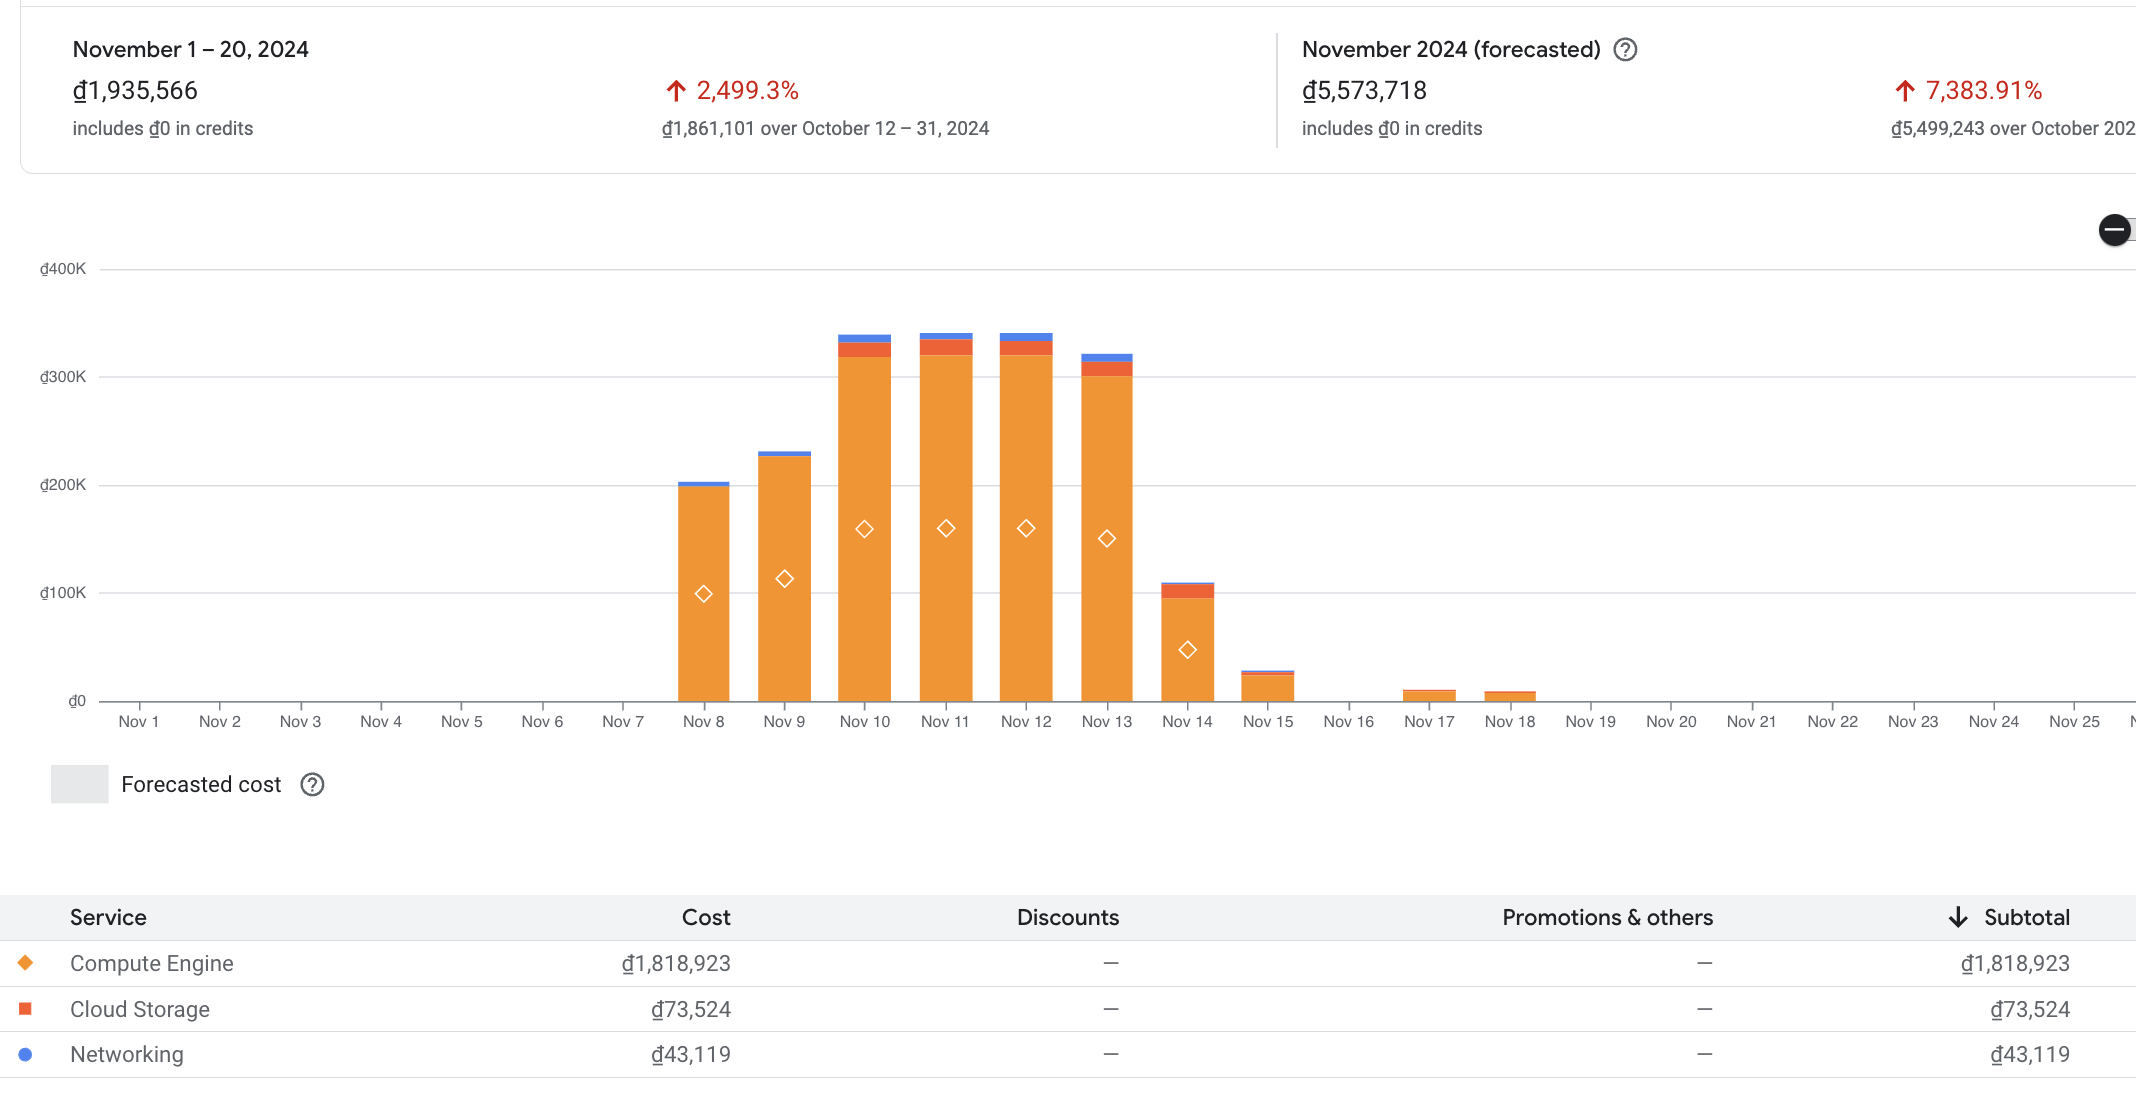
\includegraphics[width=0.8\linewidth]{images/billing.png}
    \caption{Billing over the month of research and development}
\end{figure}

The strategic implementation of IaC resulted in a substantial reduction of operational expenditures,
with costs now directly correlated to active computational requirements. This approach introduces a
level of financial granularity previously unattainable in traditional infrastructure management
models. By enabling real-time scaling and immediate resource deallocation, organizations can achieve
unprecedented levels of computational efficiency and cost control.

Comparative analysis suggests that leveraging BigQuery for data ingestion and transformation
presents a more economically advantageous approach compared to traditional Spark deployment models.
This advantage extends beyond immediate cost considerations, encompassing broader technological and
operational benefits. The combination of flexible pricing, robust infrastructure, and dynamic
resource allocation demonstrates the potential for significant optimization in complex data
engineering environments.

The evolving landscape of cloud computing and data infrastructure demands a sophisticated approach
to cost management that transcends traditional procurement methodologies. Organizations must develop
nuanced strategies that balance technological capabilities, operational requirements, and economic
constraints. Our research underscores the importance of adaptive infrastructure models that can
respond dynamically to changing computational needs while maintaining stringent economic discipline.

By adopting a strategic approach to infrastructure management, organizations can achieve a delicate
balance between technological innovation and financial prudence. The future of data engineering lies
not merely in technological capability, but in the ability to deploy these capabilities with
economic intelligence and strategic foresight.

